%; whizzy chapter -dvi
% -initex iniptex -latex platex -format platex -bibtex jbibtex -fmt fmt
% 以上 whizzytex を使用する場合の設定。
 
%     Tokyo Debian Meeting resources
%     Copyright (C) 2012 Junichi Uekawa
%     Copyright (C) 2011 Nobuhiro Iwamatsu

%     This program is free software; you can redistribute it and/or modify
%     it under the terms of the GNU General Public License as published by
%     the Free Software Foundation; either version 2 of the License, or
%     (at your option) any later version.

%     This program is distributed in the hope that it will be useful,
%     but WITHOUT ANY WARRANTY; without even the implied warranty of
%     MERCHANTABILITY or FITNESS FOR A PARTICULAR PURPOSE.  See the
%     GNU General Public License for more details.

%     You should have received a copy of the GNU General Public License
%     along with this program; if not, write to the Free Software
%     Foundation, Inc., 51 Franklin St, Fifth Floor, Boston, MA  02110-1301 USA

%  preview (shell-command (concat "evince " (replace-regexp-in-string "tex$" "pdf"(buffer-file-name)) "&"))

%%ここからヘッダ開始。

\documentclass[mingoth,a4paper]{jsarticle}
\usepackage{monthlyreport}
% 日付を定義する、毎月変わります。
\newcommand{\debmtgyear}{2014}
\newcommand{\debmtgmonth}{02}
\newcommand{\debmtgdate}{15}
% started from zero:
% (let ((year 2013) (month 7)) (+ (* (- year 2005) 12) month -1))
\newcommand{\debmtgnumber}{109}

\begin{document}

\begin{titlepage}
\thispagestyle{empty}
% タイトルページ:編集必要な部分は最初のマクロに飛ばすこと

\vspace*{-2cm}
第\debmtgnumber{}回 東京エリア Debian 勉強会資料\\
\hspace*{-2cm}

\includegraphics{image2012-natsu/dotdeb.pdf}\\
\hfill{}\debmtgyear{}年\debmtgmonth{}月\debmtgdate{}日

% ここはアップデートすること
% 全角文字にしないとフォントのサイズが合わないので注意
\rotatebox{10}{\fontsize{32}{32} {\gt 特集:dnsmasq}}\\

\vspace*{-2cm}
\hfill{}
\includegraphics[height=6cm]{image200502/openlogo-nd.eps}
\end{titlepage}

\newpage

\begin{minipage}[b]{0.2\hsize}
 \definecolor{titleback}{gray}{0.9}
 \colorbox{titleback}{\rotatebox{90}{\fontsize{80}{80} {\gt デビアン勉強会} }}
\end{minipage}
\begin{minipage}[b]{0.8\hsize}
\hrule
\vspace{2mm}
\hrule
\begin{multicols}{2}
\tableofcontents
\end{multicols}
\vspace{2mm}
\hrule
\end{minipage}

\dancersection{事前課題}{野島 貴英}

今回の事前課題は以下です:
\begin{enumerate}
 \item 本日、何の作業をやるかを宣言ください。
\end{enumerate}
この課題に対して提出いただいた内容は以下です。
\begin{multicols}{2}
{\small
\begin{prework}{ 吉野(yy\_{}y\_{}ja\_{}jp) }
\begin{itemize}
\item DDTSS
\item manpages-ja (まだ片付けられてないです...)
\end{itemize}
\end{prework}

\begin{prework}{ dictoss(杉本 典充) }

前回の続きを行う予定です(mpd5をkfreebsdで動くようにデバッグする)

\end{prework}

\begin{prework}{ Yosuke }
cl-quicklispパッケージを理解する。
\end{prework}

}
\end{multicols}

\dancersection{Debian Trivia Quiz}{野島 貴英}

ところで、みなさん Debian 関連の話題においついていますか?Debian関連の話
題はメーリングリストをよんでいると追跡できます。ただよんでいるだけではは
りあいがないので、理解度のテストをします。特に一人だけでは意味がわからな
いところもあるかも知れません。みんなで一緒に読んでみましょう。

今回の出題範囲は\url{debian-devel-announce@lists.debian.org} や \url{debian-devel@lists.debian.org}に投稿された
内容などからです。

\begin{multicols}{2}
%; whizzy-master ../debianmeetingresume201311.tex
% $B0J>e$N@_Dj$r$7$F$$$k$?$a!"$3$N%U%!%$%k$G(B M-x whizzytex $B$9$k$H!"(Bwhizzytex$B$,MxMQ$G$-$^$9!#(B
%

\santaku
{$B@hF|!"<!4|(BDebian$B$N%P!<%8%g%s$G$"$k(BJessie$B$K$F!"$H$"$k%"!<%-%F%/%A%c$N%5%]!<%H$,BG$A@Z$i$l$^$7$?!#$=$l$O!"$I$N%"!<%-%F%/%A%c!)(B}
{hurd-i386}
{s390x}
{ia64}
{C}
{$BD9$$4V$*Hh$l!*!d(Bia64$B!#(BAMD$B$N@oN,$KIi$1$?!"@$4V$KIi$1$?!#$H$3$m$G!"(Bhurd-i386$B%"!<%-%F%/%A%c$H(Bsparc$B%"!<%-%F%/%A%c$b!"(BRelease Team$B$K$h$l$P$o$j$H33$C$W$A$J>u67$N$h$&$G$9!#;29M!'(B\url{https://lists.debian.org/debian-devel-announce/2014/01/msg00008.html}}

\santaku
{$B:#7n(B2$B7n$"$?$^$K%j%j!<%9$5$l$?(Bstable$BHG$N(BDebian$B$N%P!<%8%g%s$O$$$/$D$G$7$g$&!)(B}
{7.3}
{7.4}
{7.5}
{B}
{wheezy$B;H$$$N?M$OAaB.%"%C%W%G!<%H$@!*:#2s$b%;%-%e%j%F%#$K4X$9$k(BBugfix$B$,<g$G$9!#(B}

\santaku
{Debian$B$N;q;:(B(Asset$B$N;v$G$9(B)$B$rG$$;$k$3$H$N$G$-$k!V?.Mj$KB-$kAH?%(B(Trusted Organization)$B!W$NDj5A$,@hF|%l%S%e!<$5$l$F$$$^$7$?!#?.Mj$KB-$kAH?%$N>r7o$KEv$F$O$^$i$J$$AH?%$O$I$l(B}
{$B8x<0(BDebian$B3+H/<T$,5o$J$$AH?%(B}
{$BAGAa$$1~Ez(B/$BBP1~$,$G$-$kAH?%(B}
{Debian$B<R2q7{>O$HBPN)$7$J$$AH?%(B}
{A}
{$B:G?7HG$O!"(B\url{https://wiki.debian.org/Teams/DPL/TrustedOrganizationCriteria}
$B$K7G:\$5$l$F$$$^$9!#$A$J$_$K!"?.Mj$KB-$kAH?%$,2?$r$9$k$N$+$NDj5A$K$D$$$F$O!"(BDebian$B%W%m%8%'%/%H7{>O$N(B9.4$B>O$K$"$j$^$9!#:#$^$GL@3N$J4p=`$,$J$+$C$?$N$+!)$H$$$&$N$,$A$g$C$H6C$-!#(B}

\santaku
{1/23$B$K(BPC$B%2!<%`$r%M%C%H$GGd$k%5!<%S%9(B(Steam)$B1?1D$GM-L>$J(BValve$B<R$,!"$$$/$D$+$N(BLinux$BBP1~$N%2!<%`$rL5NA$GDs6!$7$^$9$H7h$a$^$7$?!#$I$s$J?M$,BP>]$G$7$g$&$+!)(B}
{$BA4(BDebian$B%f!<%6(B}
{$BA4(BDebian$B8x<03+H/<T(B}
{$BA4(BIT$B4k6H$N(BDebian$B%5!<%P!<@o;N(B}
{B}
{$B$3$l$b%3%_%e%K%F%#$X$N4k6H$N4sIU$NJ}K!$H$7$FLLGr$$$H;W$$$^$7$?!#(B}


\santaku
{Debian$B$N8xJs%A!<%`$,!"%=!<%7%c%k%a%G%#%"$N8x<0%"%+%&%s%H$G$NH/8@$9$kFbMF$NJg=8$r$7$F$$$^$9!#:G=i$KEj9F$5$l$k$N$O$I$N%"%+%&%s%H$G$7$g$&$+!)(B}
{twitter$B$N(Bdebian}
{google$B!\$N(Bdebian}
{identi.ca$B$N(Bdebian}
{C}
{debian$B$N%=!<%7%c%k%a%G%#%"$N8x<0%"%+%&%s%H$+$i(BDebian$B$N3hF0$r%"%T$j$?$$?M$O1~Jg$7$F$_$k$HNI$$$H$*$b$$$^$9!#(B\url{https://wiki.debian.org/Teams/Publicity/Identica}}




\end{multicols}

\dancersection{最近のDebian関連のミーティング報告}{野島 貴英}

\subsection{東京エリアDebian勉強会108回目報告}

 東京エリアDebian勉強会108回目は(株)スクウェア・エニックスさんで開催されました。
5名の参加者がありました。

\begin{itemize}
\item 野島さんが、Debian Pure Blendの紹介と、Debianの公式パッケージに含まれているビジュアルノベルゲーム用のパッケージを例に用い、Pure Blend用パッケージの作り方を紹介しました。
\item 参加者全員で、各自の作業を行い、最後に成果発表をしました。
\end{itemize}

 作業ははかどったかと思います。また、最後の成果発表にて、アイデア共有とか、課題について語るなど、いろいろ盛り上がったと思いました。

 宴会は会場近くのタイ居酒屋「トンタイ」にて行いました。

% % (query-replace-regexp "<.*?>" "")
% % (query-replace-regexp "^[	 ]\+" "")

%-------------------------------------------------------------------------------
\dancersection{Debianでdnsmasqを使う}{野島 貴英}
%-------------------------------------------------------------------------------
\index{debian-dnsmasq}

\subsection{はじめに}

 dnsmasqとは、pxe/bootp/dhcp/tftp/dnsフォワーダ/dnsサーバーを一手に引き受ける事ができる便利かつ小さなソフトウェアです。こちらがあれば、仮想環境を使ったdebianシステムのデバッグ、複数のdebian環境が必要となるような開発環境構築などにとても便利です。

 ここでは、debianにて、dnsmasqを導入し、いろいろな使い方をしてみます。

\subsection{前提知識}

 過去の東京エリアDebian勉強会のKDE開発環境の資料
\cite{kde-devel-debian}を見ておくとスムーズです。こちらに、本発表にて
多数出てくる、br0デバイスをセットアップについて記載しています。

\subsection{DNSフォワーダとして使う}

 ノートPCに入れたDebian上にて、KVM/bridgeを使い、複数ホストで構成されるLAN環境を作って何か開発をすることを想定します。当然ノートPCはモバイル利用が主になりますので、モバイル用の通信アダプタを繋いだり、free wifiスポットのある喫茶店へ行ったり、東京エリアDebian勉強会でハックしたり、有線繋いだりと、いろいろなグローバル回線のある環境へ接続できる必要があります。

 ここで問題になるのは環境によって様々に変わるDNSリゾルバの扱いとなります。仮想環境上のDebianのDNSリゾルバのアドレスは、ノートPCをどこに繋ぐかによらず、一定のアドレスであると、とても便利です。こういった環境を作るのにdnsmasqは便利です(図\ref{fig:vm-env1}、図\ref{fig:vm-env2}参照。)

\begin{figure}[H]
\begin{center}
 \includegraphics[width=0.5\hsize]{image201402/vm-dns-env.eps}
 \caption{dnsフォワーダが無い場合}\label{fig:vm-env1}
\end{center}
\end{figure}

\begin{figure}[H]
\begin{center}
 \includegraphics[width=0.5\hsize]{image201402/vm-dns-env2.eps}
 \caption{dnsフォワーダがある場合}\label{fig:vm-env2}
\end{center}
\end{figure}

 では早速使ってみます。

\begin{description}
\item[Step 1.] dnsmasqを導入します。
\begin{commandline}
note-pc$ sudo aptitude install dnsmasq
\end{commandline}
%$
\item[Step 2.] br0のみlistenするようにし、dnsフォワーダとしてのみ動作するように設定します。
\begin{commandline}
note-pc$ sudo vi /etc/dnsmasq.d/forwarder.conf
interface=br0
no-dhcp-interface=br0
bind-interfaces
\end{commandline}
%$

\item[Step 3.] dnsmasqをリスタートします。
\begin{commandline}
note-pc$ sudo service dnsmasq restart
\end{commandline}
%$

\item[Step 4.] 動作を確かめます
\begin{commandline}
特定のポートだけでListenしていることを確かめる
note-pc$ sudo netstat -nlp | fgrep dnsmasq
tcp  0 0 127.0.0.1:53  0.0.0.0:*   LISTEN      16955/dnsmasq   
tcp  0 0 192.168.0.1:53  0.0.0.0:* LISTEN      16955/dnsmasq   
udp  0 0 127.0.0.1:53    0.0.0.0:*             16955/dnsmasq   
udp  0 0 192.168.0.1:53  0.0.0.0:*             16955/dnsmasq   
実際にdnsmasqを指定して名前を引いてみる
note-pc$ sudo aptitude install dnsutils
note-pc$ dig @192.168.0.1 www.debian.org a
; <<>> DiG 9.9.3-rpz2+rl.13214.22-P2-Debian-1:9.9.3.dfsg.P2-4 <<>> @192.168.0.1 www.debian.org a
; (1 server found)
;; global options: +cmd
...中略...
;; ANSWER SECTION:
www.debian.org.		300	IN	A	5.153.231.4
www.debian.org.		300	IN	A	128.31.0.51
www.debian.org.		300	IN	A	130.89.148.14
...中略...
\end{commandline}
%$
\end{description}

非常に簡単にDNSフォワーダとしてセットアップ出来ます。

また、グローバル回線を変更した場合(例:拠点Aのwifiスポットから、拠点Bのwifiスポットへ移動した等)は、
\begin{commandline}
...グローバル回線を有効にして...
note-pc$ sudo service dnsmasq restart
\end{commandline}
%$
するだけで、新しいリゾルバ先をdnsmasqは取り込み、名前解決が出来るようになります。

\subsection{簡易DNSサーバーとして使う}

 今度は単一のドメインのホストレコードを返す簡単なDNSサーバーが
ちょっと欲しくなる時があります。このような場合、dnsmasqは
簡易DNSサーバーとしてもあっさり動作させることができます。

 実はdnsmasqはデフォルトで/etc/hostsを読み込み、DNSサーバーとしても
動作しています。そのため、簡易DNSサーバーとして利用する場合、
/etc/hostsをそのまま利用するのが一番簡単です。

\begin{description}
\item[Step 1.] /etc/hostsに名前解決したいホストを書きならべる。
\begin{commandline}
#例となります。
note-pc$ sudo vi /etc/hosts
-----------/etc/hostsここから---------------
192.168.0.3 debian0
192.168.0.4 debian1.my-domain debian1
192.168.0.5 debian2.my2-domain debian2
-----------/etc/hostsここまで---------------
\end{commandline}
%$
\item[Step 2.] dnsmasqをrestartします。
\begin{commandline}
note-pc$ sudo service dnsmasq restart
\end{commandline}
%$
\item[Step 3.] 実際にDNSを引いて確かめてみます。
\begin{commandline}
note-pc$ dig @192.168.0.1 debian0 +short
192.168.0.3 (←正しく返却されている)
note-pc$ dig @192.168.0.1 debian1.my-domain +short
192.168.0.4 (←正しく返却されている)
note-pc$ dig @192.168.0.1 debian2.my2-domain +short
192.168.0.5 (←上とは異なるドメイン所属のレコードも正しく返却されている)
note-pc$ dig @192.168.0.1 debian2 +short
192.168.0.5 (←ホスト名だけでも正しく返却されている)
\end{commandline}
%$
\end{description}

\subsection{簡易PXEブートをさせてみる}

 dnsmasqを使ってpxeブートを仮想化環境であるKVMから行ってみます。
ここでは、文献\cite{pxe-boot}の方法を使い、実際にwheezyのnetinst用
インストーラが立ち上がるまで確かめてみます。

\begin{description}
\item[Step 1.] /etc/dnsmasq.d/にて、今まで書いたファイルを一旦消去(適宜)
\begin{commandline}
note-pc$ sudo rm -f *
\end{commandline}
%$
\item[Step 2.] pxeboot用の定義を記載
\begin{commandline}
note-pc$ sudo vi /etc/dnsmasq.d/pxeboot.conf
----- pxeboot.confの中身-----
interface=br0
bind-interfaces
dhcp-range=192.168.0.129,192.168.0.254,255.255.255.0,1h
dhcp-boot=pxelinux.0,pxeserver
pxe-service=x86PC, "Install Linux", pxelinux
enable-tftp
tftp-root=/home/your/srv/tftp
----- pxeboot.confの中身-----
\end{commandline}
%$
\item[Step 3.] pxeブートさせるイメージを展開しておく。
\begin{commandline}
note-pc$ cd /home/your/
note-pc$ mkdir srv;mkdir tftp
note-pc$ cd srv/tftp
note-pc$ wget http://ftp.debian.or.jp/debian/dists/stable/main/installer-amd64/current/images/netboot/netboot.tar.gz
note-pc$ tar xzf netboot.tar.gz
\end{commandline}
%$
\item[Step 4.] dnsmasqを再起動
\begin{commandline}
note-pc$ sudo service dnsmasq restart
\end{commandline}
%$
\item[Step 5.] virt-installコマンド経由で、pxeブートしてみる。
\begin{commandline}
note-pc$ sudo qemu-img create -f raw /var/lib/libvirt/images/debian-pxe 5G
note-pc$ sudo virt-install --connect=qemu:///system -n debian-pxe --ram 512 \
           --pxe --disk /var/lib/libvirt/images/debian-pxe,bus=virtio,size=5,format=raw,cache=writeback \
           --bridge=br0,model=virtio --vnc --hvm --accelerate
\end{commandline}
%$
\end{description}

 virt-viewerがすぐに開き、PXEブートして、Debian wheezyのインストール画面が出てきます。

\subsection{終わりに}

 今回ここでは、簡易dnsフォワーダ、簡易dnsサーバー、簡易pxeサーバー
をdnsmasqを使って組み立てました。

 しかし、man dnsmasqを読むと判る通り、もっと複雑な事も簡単に出来ます。
また、自分はまったく未評価ですが、最近ではlua言語と合わせて使う事ができるようです。

 複数の仮想環境を使ってノートPC上に複数のDebianの開発環境を立ち上げる場合に、
非常に便利です。dnsmasqをぜひ一度お試しあれ。

\begin{thebibliography}{0}
  \bibitem{kde-devel-debian}
    {\footnotesize{
       野島 貴英,「Debian開発者のKDE環境あれこれ」,第85回東京エリアDebian勉強会資料,
       \url{http://tokyodebian.alioth.debian.org/pdf/debianmeetingresume201202.pdf}
       }}
  \bibitem{pxe-boot}
    {\footnotesize{
       Debian.org,``PXEBootInstall'',
       \url{https://wiki.debian.org/PXEBootInstall}
       }}
\end{thebibliography}


%-------------------------------------------------------------------------------
\dancersection{会場での無線LANのつなぎ方}{野島 貴英}
%-------------------------------------------------------------------------------
 \subsection{はじめに}

 今回試験として、会場側でフィルタ無しのグローバル回線を用意しました。
ただ、会場側のセキュリティポリシーにより、
wpa-psk AES hidden SSIDという方式での提供となります。

 以下にDebianマシンでの接続方法を記載します。

 また、自分の環境では違うやり方でつながったという方は、野島まで
教えて下さい。こちらでもノウハウとして溜めていく予定です。

 \subsection{wpasupplicant及び/etc/network/interfacesを利用の場合}

 もっとも良いマニュアルは、/usr/share/doc/wpasupplicant/README.Debian.gz
となります。困った場合はこちらも合わせてご参照下さい。

 以下に/etc/network/interfacesの定義について会場の例を記載します。

\begin{commandline}  
$ sudo aptitude install wpasupplicant
# hidden ssidの元では必ず ap-scan 1,scan-ssid 1を指定する事。
# 参考:http://bugs.debian.org/358137
$ sudo vi /etc/network/interfaces
-----以下のエントリを追記ここから----------
iface wlan_tokyodebian inet dhcp
     wpa-ssid <<会場のSSID>>
     wpa-psk  <<会場のパスワード>>
     wpa-ap-scan 1
     wpa-scan-ssid 1
     
-----以下のエントリを追記ここまで----------
# 無線LANを有効にする。
$ sudo ifup wlan0=wlan_tokyodebian
# 無線LANを無効にする。
$ sudo ifdown wlan0
\end{commandline}
%$

 また、ハマってしまった時のデバッグ方法は、/usr/share/doc/wpasupplicant/README.Debian.gz中の''4. Trubleshooting''の章が便利です。

 \subsection{その他の無線LAN用パッケージを利用の場合}

 すみません、自分が情報を持たないため、現場で教えて下さい。

\printindex

\cleartooddpage

\vspace*{15cm}
\hrule
\vspace{2mm}

\includegraphics[width=2cm]{image200502/openlogo-nd.eps}
\noindent \Large \bf Debian 勉強会資料\\
\noindent \normalfont \debmtgyear{}年\debmtgmonth{}月\debmtgdate{}日 \hspace{5mm}  初版第1刷発行\\
\noindent \normalfont 東京エリア Debian 勉強会 (編集・印刷・発行)\\
\hrule

\end{document}
